\documentclass[12pt]{article}

\usepackage{sbc-template}

\usepackage{graphicx,url}

\usepackage{float}
\usepackage[utf8]{inputenc}  

     
\sloppy

\title{(Algo nesse sentido) Utilização de transitividade e simetria para geração de dados}

\author{Alison Sassi\inst{1}, Gustavo Spiess\inst{2} }

\address{Departamento de Ciências Exatas e Engenharias\\
Universidade Regional do Noroeste do Estado do Rio Grande do Sul
  (UNIJUÍ)\\
  Rua do Comércio, 3000, Universitário -- 98700-000 -- Ijuí -- RS -- Brazil
  \email{\{alisonsassij,gspiess\}@gmail.com}
}

\begin{document} 

\maketitle

\section{RESUMO}

Nos últimos cem anos, a maior pandemia ocasionado pela doença da COVID19 em 2020 foi a mais mortal, presenciamos um cenário do colapso da estrutura hospitalar pública, falta de leitos, de respiradores e profissionais da saúde. Os leitos de Unidade de Terapia Intensiva (UTI) foram alocados na sua totalidade, nesse momento os médicos tiveram um enorme desafio de entender a prioridade de um paciente em um leito de UTI, ocasionando em problemas psicológicos, muitas vezes sendo uma escolha baseado no emocional do médico. Durante esse período, médicos realizaram uma decisão de quem ocupava um leito disponível, utilizando protocolos de triagem e guias criados por vários lugares do mundo para salvar mais vidas. Dentre muitos protocolos, foi publicado em 2020 pela Associação de Medicina Intensiva Brasileira (AMIB) um protocolo que inclui um modelo de triagem para um auxílio prático aos profissionais de saúde diante de decisões complexas associadas a alocação de leitos de UTI e ventiladores. Este artigo tem por objetivo descrever o modelo publicado pela AMIB utilizado para a triagem, explicar a forma que as variáveis foram extraídas e demonstrar a criação da geração de uma base de dados para uma validação dos dados com médicos especialistas.

\textbf{Palavras-chave:} Unidade de Terapia Intensiva (UTI). Escassez de leitos hospitalares. Auxílio médico. Triagem. Protocolo.

\section{ABSTRACT}

\textbf{Keywords:} Intensive Care Unit (ICU). Shortage of hospital beds. Medical assistance. Hospital management. Protocol.

\section{INTRODUÇÃO}

Em 31 de dezembro de 2019, uma grave pneumonia de origem desconhecida na província de Hubei, em Wuhan na China, foi reportada à Organização Mundial de Saúde (OMS), após dois meses, a OMS nomeou a síndrome respiratória aguda grave como "Covid-19" causada pelo novo vírus Sars-CoV-2 transmitida em alguns países europeus \cite{sa2020especial}.

Em fevereiro do ano de 2020 foi registrado o primeiro caso no Brasil, com o nível de ameaça global muito elevado no mundo todo, assim se tornando a maior pandemia dos últimos cem anos.
Por ser uma doença facilmente contagiosa, através de gotículas de saliva, e sendo constantemente modificada geneticamente, os casos aumentaram exponencialmente em todos os estados do Brasil, ocasionando problemas respiratórios resultando em internações de Unidade de Terapia Intensiva (UTI).

O Conselho Federal de Medicina (CFM) aponta a necessidade de 1 a 3 leitos de UTI para cada 10 mil habitantes, tendo como base a indicação da Associação de Medicina Intensiva Brasileira \cite{domingues2018numero}. De acordo com o Conselho Federal de Medicina, no ano de 2018, 21.500 leitos de UTI no Brasil foram disponibilizados pelo Sistema Único de Saúde (SUS) \cite{cfm2018,cfm2020}, ainda mais com a oferta de leitos de UTI que é historicamente escasso no Brasil pelo seu alto custo \cite{murthy2015intensive}. No ano de 2020 com a alta quantidade de novos casos de COVID-19 foram disponibilizados 3.104 novos leitos apenas para leitos de UTI SUS \cite{cotrim2020crescimento}.

Diante da estrutura hospitalar precária em hospitais públicos, os leitos de UTI ficaram escassos rapidamente, o que ocasionou muitas mortes por falta de recursos. Os profissionais de saúde na linha de frente de atendimento se depararam com o fato de uma escassez de recursos para um grande número de indivíduos necessitados deles. Surge-se então o acionamento de protocolos para a triagem para uma minimização de mortes devido à doença. A não utilização de protocolos implicaria em situações absurdamente imorais, tais como a chegada do recurso escasso por ordem de entrada ou mesmo sorteio ou ainda a não oferta do recurso para ninguém \cite{costa2020protocolos}.

Um protocolo publicado em 2020 pela Associação de Medicina Intensiva Brasileira trouxe algumas regras pensadas pela equipe médica para serem eticamente defensíveis, garantindo que processos de alocação de recursos em esgotamento não ocorram em segredo, sem registro apropriado e de maneira subjetiva e inconsistente. O protocolo surgiu para que as escolhas médicas sejam claras, transparentes, tecnicamente bem embasados, eticamente justificados e que estejam alinhados ao arcabouço legal brasileiro \cite{kretzer2020protocolo}.


\section{Associação de Medicina Intensiva Brasileira (AMIB)}

Em momentos não pandêmicos, os serviços em saúde de oferta de leitos de UTI, são baseados na necessidade de terapias de suporte orgânico e probabilidade de recuperação não havendo protocolos de triagem de pacientes. Nesse cenário, quando não há escassez de leitos de UTI, o médico deve levar em consideração que a utilização do recurso tenha um benefício prognóstico das terapias, não sendo considerada uma infração ética ou legal que medidas de suporte orgânico não sejam oferecidas a pacientes que se encontram em final de vida, sendo uma decisão compartilhada entre a equipe assistente, paciente e familiares, de maneira a refletir não apenas aspectos clínicos mas também os valores e desejos dos envolvidos, respeitando à dignidade intrínseca de cada pessoa recebendo cuidados que tenham como objetivo oferecer a melhor qualidade de sobrevida, incluindo controle impecável de sintomas e acolhimento das necessidades emocionais, sociais e espirituais tanto do paciente quanto de seus familiares.

No cenário pandêmico como aconteceu no ano de 2020, provocando o indesejável esgotamento dos recursos de leitos de UTI e de ventiladores mecânicos, não foi possível aplicar em todos os casos uma decisão compartilhada com os envolvidos devido à incerteza do conhecimento do vírus como também a grande quantidade de casos simultâneos e sobrecarga nas equipes de saúde. Diante da situação colocada da responsabilidade de haver preparo para a possibilidade de racionamento de recursos
esgotados, estamos propondo um protocolo que inclui um modelo de triagem que tem como objetivo auxílio prático aos profissionais de saúde diante de decisões complexas associadas a alocação de leitos de UTI e
ventiladores.


Entre outros, um dos objetivos do Protocolo AMIB de alocação de recursos em esgotamento durante a pandemia por COVID-19 é retirar das mãos de profissionais que estão na linha de frente do cuidado a responsabilidade de tomar decisões emocionalmente exaustivas e que possam aumentar os já elevados riscos de problemas de saúde mental provocados pela pandemia da COVID-19 e consequentemente comprometer a capacidade para o trabalho a curto e longo prazo.

Profissionais da saúde desejam conduzir seus trabalhos moralmente. Tomar decisões de grande peso moral de maneira subjetiva e sem apoio institucional ou de recomendações formais pode ser emocionalmente debilitante.

A responsabilidade quanto aos princípios que devem guiar decisões de alocação de recursos escassos, portanto, ao envolver questões de justiça distributiva deve ser idealmente compartilhada com as autoridades competentes

Somam-se as preocupações com potenciais questionamentos jurídicos relacionadas às decisões e que também podem aumentar os riscos de danos à saúde mental dos profissionais.

A utilização de um protocolo de maneira consistente pelas diversas instituições de saúde garante que um maior número de pacientes sejam igualmente sujeitos aos mesmos critérios chancelados pelas autoridades responsáveis tanto pelo zelo técnico-científico quanto o ético-legal do processo.


\section{Calculos do Amib }

\begin{figure}[!htb]
    \centering
    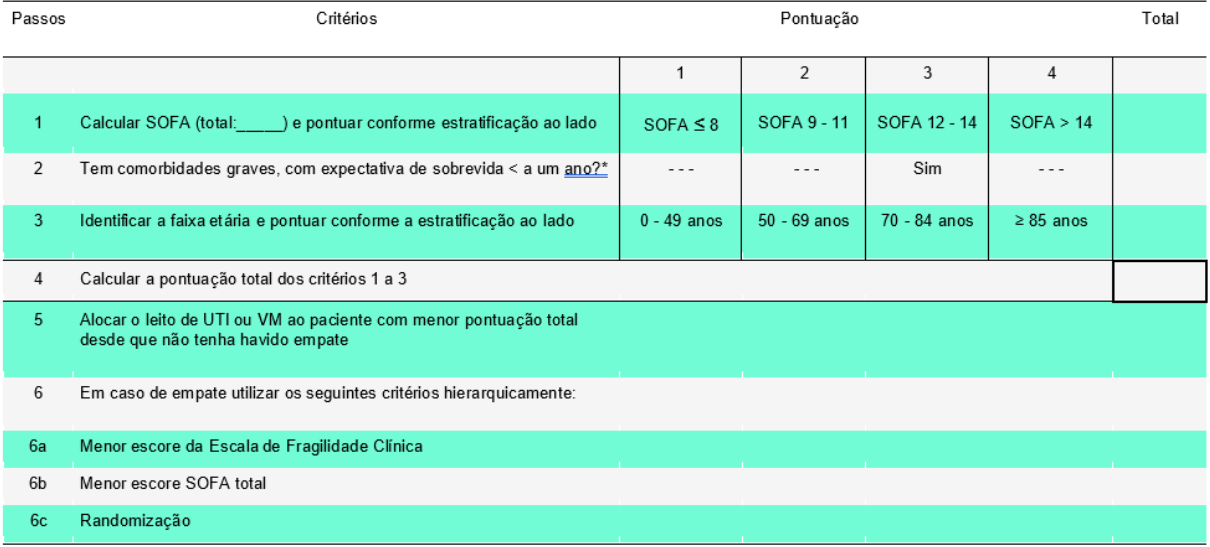
\includegraphics[scale=0.9]{img/Tabela de pontuacoes e criterios.png}
    \centering
    \caption{Calculo de pontuação e critério de desempate do modelo de triagem AMIB.}
    \label{subexpressao}
\end{figure}

O SOFA (abreviação para Sequential Sepsis-related Organ Failure Assessment), originalmente derivado de um estudo de coorte com 1449 pacientes internados em UTIs de 16 países nos anos 90, avalia objetivamente o avanço de uma disfunção orgânica em pacientes que apresentam alguma infecção, bem como a mortalidade diante de um estado de saúde crítico de um indivíduo.
O SOFA avalia 6 sistemas diferentes a partir de diversos exames clínicos e laboratoriais, e prediz a mortalidade de pacientes com sepse a partir da pontuação.

A tabela 1 demonstra a relação entre a pontuação no SOFA e a mortalidade:
PONTUAÇÃO SOFA	MORTALIDADE EM X%
0–6	<10\%
7–9	15–20\%
10–12	40–50\%
13–14	50–60\%
15	>80\%
15–24	>90\%

Esse score é baseado em seis diferentes variáveis, que avaliam os sistemas respiratório, cardiovascular, hepático, renal, neurológico e de coagulação. A cada sistema é atribuída uma pontuação de 0 (classificado como dentro dos parâmetros de normalidade) e 4 (alto grau de disfunção), totalizando um máximo de 24 pontos. A pontuação deve ser calculada 24 horas após a admissão e a cada 48 horas depois — justificando o termo “sequencial” do nome da pontuação.


SISTEMA RESPIRATÓRIO: é avaliado a partir da razão entre PaO2/FiO2, a partir de dados obtidos através de gasometria arterial. Essa razão é dada em milímetros de mercúrio (mmHg) e é considerada sem alterações quando seu valor está acima de 400mmHg. Abaixo de 400, 1 ponto no SOFA. Abaixo de 300, 2 pontos. A pontuação é 3 quando o paciente está em suporte ventilatório com a PaO2/FiO2 abaixo de 200, e ele recebe a pontuação máxima quando a relação tem resultado menor que 100mmHg com suporte ventilatório.

COAGULAÇÃO: é avaliada a partir do plaquetograma. O valor considerado de referência, ou seja, que não pontua no score SOFA, é 150.000/mm³. Os valores de corte para as pontuações de 1 a 4, respectivamente, são abaixo de 150, 100, 50 e 20. 

AVALIAÇÃO HEPÁTICA: realizada com o exame de bilirrubinas totais, que é considerado dentro dos valores de normalidade quando está abaixo de 1,2mg/dL.

SISTEMA CARDIOVASCULAR: o paciente que apresenta hipotensão e necessidade de droga vasoativa (DVA) é quem pontua nesta parte do score. É mensurado a partir da pressão arterial média, que recebe 1 ponto em caso de PAM<70mmHg. A partir do 2º ponto, é considerado o uso de DVA – 2 pontos se uso de dopamina<5 ou dobutamina em qualquer dose;  3 pontos em caso de uso de dopamina, noradrenalina ou adrenalina em doses mais baixas, e em caso de aumento da dosagem das DVAs, o paciente recebe a pontuação de 4 pontos.

SISTEMA NEUROLÓGICO: recebe avaliação a partir da escala de coma de Glasgow, conforme tabela 2. 
SISTEMA RENAL: é avaliado por dois parâmetros – creatinina e o débito urinário (a partir de 3 pontos). A creatinina se demonstra alterada a partir de 1,2mg/dL, pontuando 1 até 1,9mg/dL. Valores de 2,0 a 3,4mg/dL pontuam 2, enquanto o paciente que apresenta diurese menor que 500 ml por dia OU creatinina de 3,5 a 4,9mg/dL pontua 3. Quando a diurese é inferior a 200 ml por dia ou a creatinina é superior a 5, o paciente recebe o score máximo. 



\section{MÉTODO CIENTÍFICO}

Trata-se de uma pesquisa exploratória/explicativa, que visa propagar para os pesquisadores a identificação do problema e na proposição de uma solução computacional para analisar dados e indicar pacientes, conforme o Protocolo AMIB de alocação de recursos em esgotamento durante a pandemia por COVID-19 escolhido \cite{kretzer2020protocolo}.
Inicialmente foi realizada uma pesquisa bibliográfica, a partir da qual os pesquisadores buscaram conhecer a área em questão, identificando as melhores alternativas de solução. Em seguida, a pesquisa se tornará experimental, a fim de obter os resultados em um software contendo o modelo e a estrutura necessária para seguir na homologação, com dados que serão inseridos. 
Para apresentar a solução de maneira científica, deve ser escolhida uma metodologia que coincide com o objetivo da pesquisa. Design Science Research, é um método científico que trabalha com artefatos informacionais eficientes, tendo hipóteses teóricas fundamentadas no estado da arte e da técnica, resultando em produção do conhecimento científico pelo rigor do processo \cite{pimentel2020design}.
Nos resultados a seguir, está explicada a fase técnica para geração dos dados que serão homologados na fase de validação do modelo computacional da pesquisa.


\section{GERAÇÃO DE DADOS}

O roteiro do código se baseará no protocolo da Associação de Medicina Intensiva Brasileira (AMIB), de alocação de recursos em esgotamento durante a pandemia por COVID-19, pois entende-se que esse protocolo pode se estender para os dias pós pandemia. O protocolo busca um alinhamento com os critérios da resolução que priorizam a maior necessidade, expectativa de benefícios e adota a recomendação de que pacientes com baixa prioridade e que estão próximos à morte recebam preferencialmente cuidados paliativos. O protocolo AMIB contribui com a aplicação da resolução na medida que oferece critérios mais objetivos de avaliação de benefícios, aliviando o profissional do peso dessa tarefa em tempos de pandemia e garantindo que elas tenham maior consistência.
O modelo usará as variáveis extraídas do protocolo AMIB, sendo elas parte do Escore de falência de órgãos (protocolo Sequential Organ Failure Assessment - SOFA), com o objetivo de levantar e ensinar para o modelo quais os fatores de risco para a vida do paciente.
Utilizará de inteligência artificial supervisionada para realizar a lista de prioridades, e com seu aprendizado constante poderá efetuar uma melhor escolha, podendo se tornar uma ferramenta de apoio ensinado pelo profissional de saúde.

\section{ETAPA DE VALIDAÇÃO}
O processo de validação proposto, é através de casos clínicos hipotéticos, elaborados por grupos de médicos com experiência na área do setor de UTI que reflitam a realidade cotidiana. Os casos deverão ser cadastrados previamente na solução e validados por um profissional da saúde. Cada caso cadastrado na base será alocado a um grupo divididos em dez registros de pacientes, podendo se repetir nos grupos, conforme a aleatoriedade de um algoritmo para que não haja influência humana.
Um ou mais grupos de pacientes  terá  um  médico  que  fará  a  listagem  ordenada por prioridade, posteriormente comparado o resultado da listagem que o modelo elegeu, finalizando com um consenso entre ambas listagens, definindo se o modelo deve ter mais um ciclo de aprendizagem.
A proposta para a validação é possuir dez médicos voluntários para participar, avaliando os casos clínicos hipotéticos, realizando a separação entre os grupos de pacientes.
Os médicos voluntários terão em mãos os dados sintéticos de pacientes, com possibilidade de visualizar com detalhes cada dado clínico, realizando a escolha da posição da listagem dos pacientes. Após a escolha o médico terá o resultado do modelo desenvolvido e por fim será realizado uma entrevista para entender a divergência de opinião com o consenso entre as listagens.

\section{RESULTADOS}

Até o momento, foram realizadas a extração dos dados do Protocolo AMIB de alocação de recursos em esgotamento durante a pandemia por COVID-19, publicação do ano de 2020, as quais foram selecionadas 9 variáveis clínicas de pacientes:
1.	Idade do paciente, variável extraída do protocolo AMIB 2020.
2.	Sintomas neurológicos, variável extraída do protocolo SOFA.
3.	Sintomas cardiovasculares, variável extraída do protocolo SOFA.
4.	Sintomas respiratórios, variável extraída do protocolo SOFA.
5.	Exames de coagulação, variável extraída do protocolo SOFA.
6.	Sintomas hepáticos, variável extraída do protocolo SOFA.
7.	Sintomas renais, variável extraída do protocolo SOFA.
8.	Avaliação do Índice de Comorbidade de Charlson (ICC), variável extraída do protocolo AMIB 2020.
9.	Avaliação da escala Performance Status do Eastern Cooperative Oncology Group (ECOG), variável extraída do protocolo AMIB 2020.
Para propor o algoritmo de aprendizado de máquina supervisionado capaz de interpretar os critérios, é necessário ter uma quantidade de dados já avaliados por especialistas. Anteriormente à etapa aprendizado de máquina, utilizou-se a linguagem de programação propósito geral, muito utilizada em atividades de análise de dados (LOPES, 2019) para gerar uma massa de dados planejada e preparada para a validação.
O pacote Faker desenvolvido para a linguagem Python, que gera nomes reais anonimizados pelo algoritmo de forma mesclada, proporcionou uma geração da massa de dados de forma simples, e eficaz, assim como o pacote Random que gera números pseudo-aleatórios conforme necessidade. Ambos utilizados para gerar uma massa de dados predefinida pelo protocolo AMIB de 2020.
Com as 6 variáveis do SOFA sendo geradas entre números inteiros entre 0 e 4, a variável ICC gerada somente nos números 2 ou 4 e por fim a variável ECOG sendo gerada entre os números 0 e 4 para pacientes que tiverem mais de 60 anos. Desta forma, a uma massa de dados gerada foi armazenada como mostra no segmento de dados abaixo:

\begin{figure}[!htb]
    \centering
    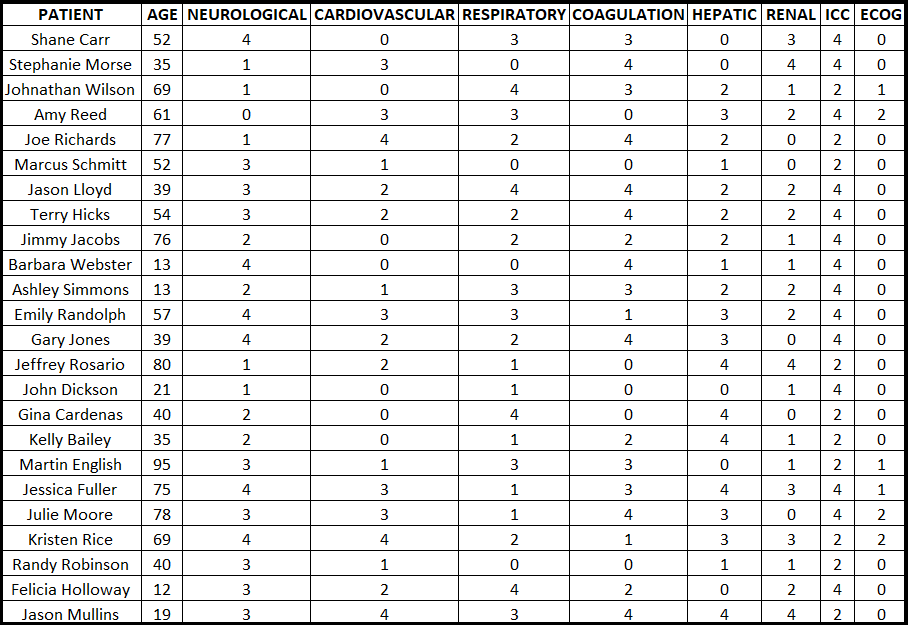
\includegraphics[scale=0.6]{img/massa de dados gerada.png}
    \centering
    \caption{Massa de dados gerada.}
\end{figure}

O modelo proposto no protocolo AMIB 2020 foi composto por um sistema de avaliação de múltiplos critérios que representam diferentes objetivos éticos: i) salvar o maior número de vidas; ii) salvar o maior número de anos/vida; iii) equalizar as oportunidades de se passar pelos diferentes ciclos da vida. O sistema de pontuação pode variar do número dois a onze, onde quanto menor é a pontuação de um paciente, maior será a sua prioridade de alocação de recursos escassos. Quanto maior o número de pacientes a serem triados, maior será a expectativa de empates nas pontuações e por esta razão o protocolo, assim como o de Biddinson et al, também inclui sugestões de critérios de desempate, os quais serão calculados juntos com a base de treinamento, para isso levantou-se os critérios. Em caso de desempate o presente modelo sugere os seguintes critérios de desempate sequenciais:
\begin{itemize}
  \item Escore de fragilidade clínica;
  \item Pontuação total do SOFA;
  \item Randomização.
\end{itemize}

Um segmento da base de dados gerado sinteticamente, o qual contém o cálculo de critérios de desempate, será utilizado para que a Rede Neural possa analisar em conjunto com os dados de cada paciente.


Com os dados gerados, foi possível criar um sistema capaz de separar em grupos definidos de dez registros, distribuídos de forma agrupada com o objetivo de que uma equipe médica possa validar a ordenação de cada grupo, entendendo qual paciente deve ter a prioridade conforme sua experiência. 
Um ou mais grupos serão compostos por dez registros hipotéticos, com as variáveis extraídas do protocolo AMIB de alocação de recursos em esgotamento durante a pandemia por COVID-19, sendo validados com um médico especialista de forma de listagem em ordem de prioridade conforme sua experiência profissional.
Será utilizada a mesma base de dados com as avaliações médicas, inserindo os dados no modelo computacional para ensinar um algoritmo de inteligência artificial a realizar uma listagem dos pacientes que estão na espera de um leito de UTI.

\section{PRÓXIMAS ETAPAS}
Após esse resultado mapeado e esperado, as próximas etapas para o desenvolvimento da aplicação proposta no projeto é propor e escrever o algoritmo de aprendizado de máquina supervisionado capaz de interpretar os critérios, realizar a validação do modelo, treinar o algoritmo com os dados dos critérios extraídos, realizar e qualificar a validação do modelo construído, reajustando se necessário.
E por fim a validação dos dados gerados com o grupo de médicos voluntários o qual será realizado por especialistas que possam validar o modelo e ensinar a rede neural com a experiência de médicos.

\section{CONSIDERAÇÕES FINAIS}
No presente trabalho tratou-se do problema de pesquisa identificado sobre a escassez de leitos de unidade de terapia intensiva, levantando uma solução para o auxílio do médico intensivista.
Foi descrito as etapas técnicas para geração de uma base de dados conforme planejamento da pesquisa que está em andamento, como também a forma de validação destes dados.
O sistema auxiliará o médico intensivista em um hospital quando os leitos de UTI estiverem escassos, utilizando um modelo computacional para geração de uma lista de pacientes.

\section{REFERÊNCIAS BIBLIOGRÁFICAS}

\bibliographystyle{sbc}
\bibliography{sbc-template}

\end{document}

